\documentclass[twoside]{report}
\usepackage[utf8]{inputenc}
\usepackage{VassorTitle}
\usepackage[super]{nth}
\usepackage{lettrine}
\usepackage{xstring}
\usepackage{todonotes}
\usepackage{graphicx}
\usepackage{tikz}
\usepackage{csquotes}


\institution{École polytechnique fédérale de Lausanne}
\project{\nth{1} semester report --- HUM-428}
\supervisor{Pr.~\textsc{Vinck}}


%\renewcommand\paragraph[1]
%{
%	\lettrine{\StrLeft #1 {1}}{\StrGobbleLeft #1 {1}}
%}
% TODO : Lettrine paragraphe

\graphicspath{{figures/}}

% Document description
\title{Proposal for a methodology of startup analysis}
\author{Giulia \textsc{Ferrari}\\Martin \textsc{Vassor}}

% Beginning document
\begin{document}
\maketitle
\begin{abstract}
	\paragraph{}
	This report is made for the HUM-428(a) course entitled \emph{Sciences,~technology~and~society}, told by Pr.~\textsc{Vinck} with Richard~\textsc{Marion} and Alexandre~\textsc{Camus} as lecturer assistants at the \textsc{École Polytechnique Fédérale de Lausanne}. Its goal is to conclude the fall semester lectures and provide a base for spring semester work. 
	
	For this purpose, it first sums up the knowledge acquired during the semester, making a link between the theoretical concepts and the interventions of external lecturers. Then, it proposes a methodology for the study case we'll do in the forthcoming semester.
\end{abstract}
\tableofcontents
\listoffigures
\listoftables
\chapter{Learned knowledge}
\section{External lecturers}
\begin{table}
\begin{tabular}{ccp{5cm}}
\textsc{Start-up} & \textsc{Innovator} & \textsc{Product} \\
Hidacs & Patrick Marmaroli & High end directional loudspeaker that diffuses light and music locally. \\
Future Instruments & Alain Crevoisier & Technology that transforms any flat surface into a tactile interface. \\
GlobalNeonat & Benjamin Rime & Incubator made of PCMs  for developing countries.\\
Artanim Interactive & Alain Renaud & Series of products based on innovative algorithms in the domain of motion capture. \\
\end{tabular}
\caption{Start-ups and their products that were examined during the sessions in class.}
\label{tab:lecturers}
\end{table}
\section{The notion of uncertainty}
\paragraph{}
Uncertainty is a notion that concerns every facet of modernity. At times it may seem inconsequential, but it could not appear more evident in the sessions during which guests spoke about their innovative ideas and start-ups (see \ref{tab:lecturers}~p.\pageref{tab:lecturers}). 
\paragraph{}
They have been invited to recount their experiences to the class, but on a deeper level they were actually talking about the numerous occasions in which they concretely came face-to-face with uncertainty. This is a common occurrence especially in the case of start-ups, whose essential nature is aptly captured by Ries (\cite{ries_what_2010}). He defines a start-up as a \begin{quote}human institution designed to deliver a new product or service under conditions of extreme uncertainty.\end{quote}
\paragraph{}
It is foremost a human enterprise because, like in any other company, the value creation is located in the people who work together to create a product out of the original idea, creative employees are hired and then must be coordinated to deliver results.  Secondly, a start-up aims to uncover a new source of value for customers, thus proposing a new product to them. The question of innovation is more delicate, since we find that even the most radical new inventions build upon previous technology. Even if we are used to think of a new product whenever innovation is mentioned, a lot of start-ups don't innovate at all in the product dimension but they base their work on repurposing an existing technology for a new use (such is the case of GlobalNeonat, that found another application for phase-change materials, integrating it into a new kind of incubator), devising a new business model or simply locating an existing product or service in an unexplored geographical area. 
\paragraph{}
However, what really distinguishes start-ups from the rest of the companies – small and large alike – is the context in which they work: one of extreme uncertainty. As Ries (\cite{ries_what_2010}) explains : \begin{quote}"startups are designed for the situations that cannot be modeled, are not clear-cut, and where the risk is not necessarily large – it's just not yet known".\end{quote} This applies to factors that can be either external – such as the existence of a market and the propensity of potential financiers to invest in the project – or internal – such as the actual feasibility of the invention, the way to conduct the development process, the amount of time and resources that should be accounted for. When success is not guaranteed, there is always a measure of risk involved and it is clear that a company for which uncertainty is not the main concern does not belong to the "start-up domain"\todo{Quote or neologism ?}.
\paragraph{}
This is also the reason why common management best practices do not apply to start-ups. For instance, the common entrepreneur is prone to think that when a new project is on track, on time and on budget it is well-managed and will lead to success. This is not true in the start-up case, since if an ardent innovator fails to understand that he is building something that in the end will not interest any kind of customer, even a perfectly conducted project will be wasted effort. This was precisely the case of Future Instruments. The founder, Mr. Crevoisier, is an ardent fan of electronic music and he devoted ten years of his life to find a way to make his idea a reality. The new technology was born out of and built on the basis of his own needs; in 2007, with the construction of the first prototype, the product was ready to be launched on the market. However, potential investors, though believing the idea held merit, responded with a rejection, as a real market – beside the inventor – didn't exist. For this same reason, Future Instruments also represents a manifest example of the so-called "innovator's four pathologies"\todo{Quote or neologism?}, at least where lack of criticism acceptance and definition of pathway and market are concerned. 
\paragraph{}
\cite{ries_is_2010}\todo{introduce the quote}
All entrepreneurs face the same fundamental challenges:
\begin{itemize}
\item How do we know if we're making progress?
\item How do we know if customers will want the product we are building?
\item And, if they do, how do we know what kind of value we can create with it? 
\end{itemize}
But because every start-up strives to become an institution and build a sustainable business, answering these questions requires progressively acquired learning and a specifically tailored kind of accounting. This can be achieved through the coordination of many different people, who must work together to find the answers. In fact, one of the aspects which the four start-ups in exam have in common is precisely teamwork. The enterprises might have originated either from a foundation spin-off, a master project in university, the university laboratory or simply from the ambitious idea of a man, but they ultimately grew to include more people who provide their expertise in various fields as well as valuable advice. \todo{Copy/paste from article : introduce the quote}
\paragraph{}
When analyzing the four different cases of start-ups, we have been able to realize that there exist as many differences as few commonalities between them. However, the background, experiences and ideas may be very different, but the overall uncertainty concerns the same aspects:
\begin{itemize}
\item market and clients;
\item product and/or project;
\item technical feasibility.
\end{itemize}
\paragraph{}
In terms of venture financing, these issues are common in enterprises that are in the "early stage"\todo{quote or idea ?} of their development cycle, which comprehends two consecutive phases: 
\begin{enumerate}
\item the seed stage: the entrepreneur focuses on fundamental R\&D activities; in the process, he inevitably faces some elementary uncertainties that are also the highest throughout all the life-cycle of the enterprise because at this point both the market acceptance and the product technical feasibility must be evaluated;
\item the start-up stage: once prototypes have been assembled and tests on the product and the market have been conducted, the entrepreneur attempts to commercialize his idea; the risks and the uncertainty are partially mitigated by the preliminary tests, while tasks start becoming numerous and complex, thus the innovator starts hiring additional staff to complement missing expertise. In this manner, he is also alleviating risks regarding the management quality \cite{eckermann_venture_2006}.
\end{enumerate}
In addition to this classification, Startup Commons gathered information from many start-ups all over the world and simplified it into a framework (see \ref{fig:framework} p.\pageref{fig:framework}) that aims to show how innovators usually develop both their ideas and a committed founding team into a real growing business that captures the value being created (\cite{commons_startup_2015}).
\begin{figure}
\begin{center}
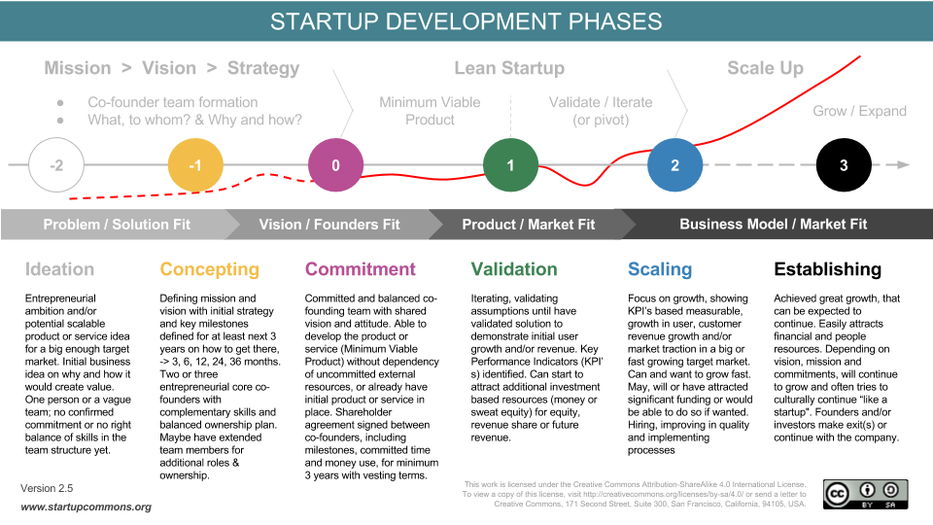
\includegraphics[width=\linewidth]{development_phases.png}
\caption{Start-up development phases \cite{startup_commons_startup_2015}.}
\label{fig:framework}
\end{center}
\end{figure}
\paragraph{}
As far as the examined four start-ups are concerned, all of them experience a certain level of uncertainty related to market. It can be connected to the definition of either the clients or the existing clients' needs (in the case of Hidacs), but it still probably represents the main concern for every newly-formed enterprise. Besides, if a client base existed for every single innovative idea, we would observe so many more start-ups transforming into successful businesses. 
We have been able to observe that usually the definition of a market is strongly correlated to the start-up's efforts in gathering feedbacks on the targeted clients' acceptance of the product.
\begin{figure}
\begin{center}
\missingfigure[figwidth=6cm]{Draw figure}
\caption{How the four start-ups in exam position themselves in terms of market definition and gathering of feedback on market acceptance activities.}
\label{fig:position}
\end{center}
\end{figure}
As \ref{fig:position} p.~\pageref{fig:position} shows, Future Instruments has major problems in this regard because of Mr. Crevoisier's lack of sufficient consideration of the customers' needs and wants in the first phase of his start-up. Consequently, he found himself in the disagreeable position of having spent a major part of his life on assertively developing a product whose customers' (still) didn't exist and of having to rapidly find another market segment to target. On the other extreme we find Hidacs and GlobalNeonat, whose client base was already clearly defined before the actual development of the product. Mr. Marmaroli admits to facing market uncertainty every day, but this is due to the difficulty in understanding more the clients' needs when dealing with a customizable product than their identity, which was already known to the Metamedia Center. The same applies to GlobalNeonat, whose main concern was evaluating the market's reception. To solve this issue, Mr. Rime went to Cameroon to interview the potential users, thus gathering direct feedbacks. Artanim Interactive represents a peculiar case, as an investigation on market acceptance was never conducted during the conception of the products, but the founder, Mr. Renaud, declares that the market is extremely varied, thus clients are sure to exist. The very difference between these last two cases may be also attributed to the different mindsets of the two innovators: on the one hand Mr. Rime adopted a cautious approach, on the other Mr. Renaud was influenced by the American way to do things that is less cautious, more encouraging and optimistic about the ideas' outcomes. 
\paragraph{}
Undoubtedly, the innovators' approaches to feedback collecting derive from their different innovation methods. In this respect, all the innovations taken in exam can be classified as \emph{technology push}, with the exception of Hidacs, which can be defined \emph{market pull}. With the first approach, the stimulus for new products and processes comes from (internal and external) research; the goal is to make commercial use of new know-how and it does not matter is a certain demand already exists or not. With the second one, though, the innovation's source is a currently inadequate satisfaction of the customers' needs, whose demands are thus articulated by willing individuals or groups of innovators \cite{brem_2009_integration}, see \ref{fig:models} p.~\pageref{fig:models}.
\begin{figure}
\begin{center}
\missingfigure[figwidth=6cm]{Draw figure}
\caption{Schematic presentation of technology push and market pull models.}
\label{fig:models}
\end{center}
\end{figure}
\paragraph{}
Although it is unlikely to find enterprises that do innovation according to one of these two extremes, it is true that a particular invention derives from an impulse that is closer to one of these two models and subsequently implicates different procedures on the innovator's part, upon which we are not going to enlarge.
\paragraph{}
When asked about the \emph{tug-of-war} between them, Dr. Erika \textsc{Wagner}, the Executive Director of the X PRIZE Lab@MIT, said \cite{awolfson_entrepreneurship_2010} : \begin{quote}Is an entrepreneur with a market need in mind and a product to fit that need better positioned for success than an entrepreneur who starts with a technology but \emph{needs} a need? I'd argue yes.\end{quote} Indeed, this reasoning is embodied in such start-ups as Hidacs and Future Instruments: whereas Mr. Marmaroli received a direct request to implement a technology, Mr. Crevoisier's success never came to be because of the lack of initial need expressed by the potential customers. This is the reason why collection of feedbacks during the development phase was not necessary in the first case, but decidedly so in the second one.
\paragraph{}
Nowadays, everyone with a good idea and an entrepreneurial proclivity has the possibility of founding an enterprise. For a student there is not even the need to own initial capital, as universities are becoming real launch pads for start-ups in every regard. They are a relatively fail-safe system, with an excellent network of contacts, diversity of ideas and opinions, financial offers, fully equipped laboratories and technical support at disposal \cite{stagars_university_2015}. Instances of this trend are Hidacs and GlobalNeonat: the first was born out of a PhD project in EPFL laboratory, the second saw Mr. Rime conducting the research on the incubator as a master project. In both cases, though, the innovative idea did not originated from them but from the university or its partners (MetaMedia Center). This had also an indirect effect on the technical feasibility. In fact, contrarily to the other two innovators' cases, Mr. Marmaroli and Rime did not have enough practical knowledge at first to embark in such a project without the assistance of professors and colleagues with practical experience in the field. As they both underlined, there was a certain level of uncertainty related to feasibility. For instance, Hidacs is currently composed of four friends that equally share risks and profits, but the technology was developed in a laboratory environment where the regular interaction with experts and individuals from various disciplines provides a fantastic vehicle for innovation. Indeed, there are not many platforms besides the university that provide such an opportunity. These people's contribution was therefore essential not only in the development of the product, but also in providing the technical and practical knowledge, together with the discipline and the work ethic, that is generally lacking in a fresh-faced student but is otherwise needed to launch a start-up. Therefore, if Mr. Rime had to face some major challenges while building the prototype for his incubators, Mr. Marmaroli has been experiencing uncertainty regarding feasibility since the product was marketed, as the clients have different tastes that make customization a requirement, which in turns increases the risk of having a final product that does not work in the way it is supposed to. On the contrary, for Future Instruments and Artanim Interactive it was never a question of feasibility, as they both could benefit from their years-long experience with working outside of the university environment. In their case, once the product is put to market, it is deemed as perfectly working.
\paragraph{}
Lastly, it is important to discuss financing. Although it is not directly related to uncertainty, it certainly has a big impact on it as it increases risks. At the initial stage of an enterprise, a lender or an investor do not exist yet, making a personal financial investment the only alternative – unless the innovator is assisted by an institution, such as the university or a foundation. The lack of founding can seriously undermine the development project, as cash is needed to buy raw material, rent facilities, make trips away from home and to pay every kind of external helpers. Furthermore, it is not even sufficient to have an innovative idea, a solid business plan and a working prototype – as Mr. Crevoisier's experience taught – but a potential investor who is aware of the risks expects the product to be ready to be sold, with a well-defined market segment. This is the reason why, in general, if money is not an issue, the uncertainty regarding an innovation can be significantly decreased.







%%%%%%%%%%%%%%%%%%%%%%%%%%%%%%%


\chapter{Description of the startup}
\section{SqeedTime}
SqeedTime is a new startup from Lausanne. Its purpose is to provide a smartphone application to enforce the link between local shops, restaurants or all kinds of professionals and the potential customers.
\marginpar{
	\begin{itemize}
		\item Spontaneous meetings
	\end{itemize}
}



\paragraph{Organization}
At first, SqeedTime was founded by Paul-Edgar \textsc{Levy} and Timothée \textsc{Barghouth}, two law students. Now, SqeeTime consists of a team of five members.
\marginpar{
	Demander les autres
}
\paragraph{History and original idea}
During summer 2014, both entrepreneurs observed that even with social networks, they couldn't organize a spontaneous meeting with friend. After this statement, they decided to create such a tool, which finally leads to the application to be released soon.
\section{Product}
\section{Activity domain}







\chapter{Kinds of uncertainty}
\section{Uncertainty related to the digital domain}
\subsection{The uncertainty in digital innovation field}
\paragraph{}
The level of uncertainty depends as much on the product as on the sector it belongs to. As far as the various activity sectors are concerned innovation may be either a necessity, common practice, welcomed or unprecedented.
\paragraph{}
In the era of digital convergence, digital content services (services that deliver content created, used, shared, accessed and preserved in a digital format) are highlighted as a driver of innovation \cite{toivonen_innovation_2007, gwee_innovation_2009}. The innovation in this sector does not only transform the existing markets, but creates an opening for new opportunities. This is made possible because of the products' unique characteristics \cite{kim_patterns_2012}:
\begin{itemize}
\item digital content services use common digital formats: a network facilitates delivery and share of all kinds of content;
\item content is edited easily and augmented using multiple available sources (mash-up in web service);
\item digital content services possess the characteristics of both product and service, so that potential of innovation is increased.
\end{itemize}
\subsection{The case of AppStores, uncertainty of distribution plateforms}
\paragraph{}
Recently, what have been highlighted as new content services are mobile applications (apps) in App Stores. Product of this kind have proliferated in the last years. The enormous growth of this sector - coupled with its low market-entry cost for developers and growing list of enviable success stories - attracted the attention of entrepreneurs, to whom Apple's App Store and the Android Market provide easy access \cite{wacheski_anystone_2011}.
\paragraph{}
However, the endless possibilities which this sector seems to offer could actually make it only fool's gold, as they increase competition and risk of failure. Among more than one million and a half of apps in the Apple App Store, getting noticed and generating substantial revenues is a great challenge for entrepreneurs, who must aim for innovation if they want to gain success.
\paragraph{}
As far as uncertainty is concerned, application developers can face uncertainty related to either market, product or feasibility. 
\paragraph{}
Regarding the first one, it is imperative to define a market for one's innovative idea, because a lack of consideration for this issue can result in unquestionable failure. Although it is true that high competition spurs innovation, an entrepreneur should always be aware of the potential customers' needs and wants, especially if his app's concept was born out of his own need and not by observing the other's. Indeed, market uncertainty is probably the one feature that all activities with a commercial goal have in common.
\paragraph{}
Despite the similarities in the types of uncertainty concerned, one of the main differences between a physical product and a digital content service is that whereas a manufacturer often handles the direct sale to the customers and can choose the best strategy to cultivate this relationship, an app developer is forced to subject to the platform's rules and constraints. The digital content is delivered from a service provider to the end user by the means of a platform, such as Apple Store, Google Play, etc. (fig. \ref{fig:content_service}~p.\pageref{fig:content_service}). This means that particular attention should be given to the choice of the store in which one intend to sell its mobile application. For instance, Apple implemented an App Review process to evaluate all submissions and filter them on the basis of some criteria, such as the replication of an already existing application or the expected reaction on the customers' side. Thus, it is evident that a major uncertainty related to the product is present, therefore a developer should be able to define the concept of his product and self-evaluate the willingness to buy it of the customers. Indeed, experiences of various start-ups revealed that the inability of some entrepreneurs to see beyond their enthusiastic confidence in their ideas ultimately brought them to denied entrance in the store and ensuing financial losses. More sensible developers, though, are able to repeatedly evaluate the product concept and their objectives, going through many iterations of trial and error to transform a great idea into a great application, even if the result is not as originally expected. \enquote{It is better to fail fast, learn, and move on quickly}, the CEOs of Anystone Technologies, a mobile applications start-up, commented in this regard.
\begin{figure}
\begin{center}
% Graphic for TeX using PGF
% Title: /home/martin/Documents/EPFL/Master/Semestre I/SHS-1/Rapport_semestre_I/figures/content_service.dia
% Creator: Dia v0.97.3
% CreationDate: Sat Dec 19 00:31:14 2015
% For: martin
% \usepackage{tikz}
% The following commands are not supported in PSTricks at present
% We define them conditionally, so when they are implemented,
% this pgf file will use them.
\ifx\du\undefined
  \newlength{\du}
\fi
\setlength{\du}{15\unitlength}
\begin{tikzpicture}[scale=2]
\pgftransformxscale{1.000000}
\pgftransformyscale{-1.000000}
\definecolor{dialinecolor}{rgb}{0.000000, 0.000000, 0.000000}
\pgfsetstrokecolor{dialinecolor}
\definecolor{dialinecolor}{rgb}{1.000000, 1.000000, 1.000000}
\pgfsetfillcolor{dialinecolor}
\pgfsetlinewidth{0.050000\du}
\pgfsetdash{}{0pt}
\pgfsetdash{}{0pt}
\pgfsetmiterjoin
\definecolor{dialinecolor}{rgb}{0.000000, 0.000000, 0.000000}
\pgfsetstrokecolor{dialinecolor}
\draw (33.000000\du,11.000000\du)--(33.000000\du,16.000000\du)--(39.000000\du,16.000000\du)--(39.000000\du,11.000000\du)--cycle;
% setfont left to latex
\definecolor{dialinecolor}{rgb}{0.000000, 0.000000, 0.000000}
\pgfsetstrokecolor{dialinecolor}
\node[anchor=south west] at (33.000000\du,11.000000\du){Digital content};
\pgfsetlinewidth{0.050000\du}
\pgfsetdash{}{0pt}
\pgfsetdash{}{0pt}
\pgfsetmiterjoin
\definecolor{dialinecolor}{rgb}{0.000000, 0.000000, 0.000000}
\pgfsetstrokecolor{dialinecolor}
\draw (33.400000\du,14.600000\du)--(33.400000\du,15.600000\du)--(38.600000\du,15.600000\du)--(38.600000\du,14.600000\du)--cycle;
% setfont left to latex
\definecolor{dialinecolor}{rgb}{0.000000, 0.000000, 0.000000}
\pgfsetstrokecolor{dialinecolor}
\node at (36.000000\du,15.10000\du){Platform};
\pgfsetlinewidth{0.050000\du}
\pgfsetdash{}{0pt}
\pgfsetdash{}{0pt}
\pgfsetmiterjoin
\definecolor{dialinecolor}{rgb}{0.000000, 0.000000, 0.000000}
\pgfsetstrokecolor{dialinecolor}
\draw (33.400000\du,11.600000\du)--(33.400000\du,13.600000\du)--(38.600000\du,13.600000\du)--(38.600000\du,11.600000\du)--cycle;
% setfont left to latex
\definecolor{dialinecolor}{rgb}{0.000000, 0.000000, 0.000000}
\pgfsetstrokecolor{dialinecolor}
\node[anchor=south west] at (33.400000\du,11.600000\du){Content};
\pgfsetlinewidth{0.050000\du}
\pgfsetdash{}{0pt}
\pgfsetdash{}{0pt}
\definecolor{dialinecolor}{rgb}{0.000000, 0.000000, 0.000000}
\pgfsetstrokecolor{dialinecolor}
\pgfpathellipse{\pgfpoint{34.800000\du}{12.600000\du}}{\pgfpoint{1.000000\du}{0\du}}{\pgfpoint{0\du}{0.600000\du}}
\pgfusepath{stroke}
% setfont left to latex
\definecolor{dialinecolor}{rgb}{0.000000, 0.000000, 0.000000}
\pgfsetstrokecolor{dialinecolor}
\node at (34.800000\du,12.600000\du){Product};
\pgfsetlinewidth{0.050000\du}
\pgfsetdash{}{0pt}
\pgfsetdash{}{0pt}
\definecolor{dialinecolor}{rgb}{0.000000, 0.000000, 0.000000}
\pgfsetstrokecolor{dialinecolor}
\pgfpathellipse{\pgfpoint{37.200000\du}{12.600000\du}}{\pgfpoint{1.000000\du}{0\du}}{\pgfpoint{0\du}{0.600000\du}}
\pgfusepath{stroke}
% setfont left to latex
\definecolor{dialinecolor}{rgb}{0.000000, 0.000000, 0.000000}
\pgfsetstrokecolor{dialinecolor}
\node at (37.200000\du,12.600000\du){Process};
\pgfsetlinewidth{0.050000\du}
\pgfsetdash{}{0pt}
\pgfsetdash{}{0pt}
\pgfsetbuttcap
{
\definecolor{dialinecolor}{rgb}{0.000000, 0.000000, 0.000000}
\pgfsetfillcolor{dialinecolor}
% was here!!!
\pgfsetarrowsend{stealth}
\definecolor{dialinecolor}{rgb}{0.000000, 0.000000, 0.000000}
\pgfsetstrokecolor{dialinecolor}
\draw (36.000000\du,13.600000\du)--(36.000000\du,14.600000\du);
}
\pgfsetlinewidth{0.050000\du}
\pgfsetdash{}{0pt}
\pgfsetdash{}{0pt}
\pgfsetbuttcap
{
\definecolor{dialinecolor}{rgb}{0.000000, 0.000000, 0.000000}
\pgfsetfillcolor{dialinecolor}
% was here!!!
\pgfsetarrowsend{stealth}
\definecolor{dialinecolor}{rgb}{0.000000, 0.000000, 0.000000}
\pgfsetstrokecolor{dialinecolor}
\draw (35.800000\du,15.600000\du)--(35.800000\du,17.600000\du);
}
\pgfsetlinewidth{0.050000\du}
\pgfsetdash{}{0pt}
\pgfsetdash{}{0pt}
\pgfsetbuttcap
{
\definecolor{dialinecolor}{rgb}{0.000000, 0.000000, 0.000000}
\pgfsetfillcolor{dialinecolor}
% was here!!!
\pgfsetarrowsend{stealth}
\definecolor{dialinecolor}{rgb}{0.000000, 0.000000, 0.000000}
\pgfsetstrokecolor{dialinecolor}
\draw (36.200000\du,17.600000\du)--(36.200000\du,15.600000\du);
}
% setfont left to latex
\definecolor{dialinecolor}{rgb}{0.000000, 0.000000, 0.000000}
\pgfsetstrokecolor{dialinecolor}
\node[anchor=north] at (36.000000\du,17.600000\du){User};
\end{tikzpicture}

\caption{Structure and components of digital content services (\cite{kim_patterns_2012})}
\label{fig:content_service}
\end{center}
\end{figure}
\paragraph{}
As for minimizing risks inherent development and feasibility, \cite{tiwana_platform_2014} suggests to schedule stages with the greatest uncertainty as late as possible in the project roadmap. Unless there is a clear first-mover advantage, at first a developer should focus on opportunities with the least technical uncertainty and the highest immediate payoff, ensuring that the benefits will begin being collected earlier rather than later. This approach can reduce challenges as well as uncertainty in the subsequent stages, as new information – regarding the market, the customers' issues and needs, further developments, etc. – can be obtained during the implementation of the preceding stages. Even if some steps of the future strategy might be never executed, at least some payoff is generated from what is feasible instead of pursuing an all-or-nothing proposition.
\paragraph{}
Analyzing the experiences of other start-ups in this sector, we can point out some of the most important aspects which an app developer should keep into account if he wants to transition into the market as smooth as possible:
\begin{enumerate}
\item \emph{App stores' differences:} the main app stores nowadays are Apple App Store, Google Play (Android), BlackBerry App World and Windows Phone App Marketplace. Each one of them has different characteristics that may suit an entrepreneur better or worse. For instance, with respect to the majorly used ones, the advantage of Google Play is the wide choice it offers and its open source model, enabling nearly anyone to add their apps. However, Android suffers from the drawback of running on many hardware platforms, which forces the developers to cover multiple designs and testing permutations. In contrast, there is a greater guarantee of quality in the Apple Store than with Android, as Apple tests and approves every app that goes on sale in the App Store. Furthermore, the exclusivity of the Apple system limits the hardware variants tremendously. This contributes to Apple Store's popularity among the mobile users, making it the most profitable for developers – if not the best choice. In addition, while Google Play allows the developers to be in direct contact with the customers and provides them with some detailed statistics about users, the Apple Store does not allow anything of all this.
\item \emph{Predominant sales model in the app store:} although an entrepreneur would like the option to choose whether his app should be available for free or for a price, he should also consider which is the predominant sales model in the chosen app store. In fact, despite the willingness of consumers to pay for a useful mobile application, if the app store encourages the sellers to include a free or \emph{lite} edition of their products with limited capabilities, this trend should not be overlooked. Consumers are reluctant to pay for an application without trying it first and making it free removes a powerful mental barrier from potential purchases, increasing revenues.
\item \emph{Price changes and promotions:} they can greatly influence download rates and sales. They become advertisement tools when there are mobile applications that monitor price drops, and should be used to prompt more reviews online and by word of mouth. Time-limited promotions are also particularly useful when the product includes a free version besides the full one. This makes advertising mostly unnecessary as the free edition's goal is already to encourage the purchase of the complete edition. Nonetheless, purchasing behavior should be well monitored to keep track of the products' sales.
\item \emph{Customers' reviews:} they are a powerful tool that can impact on sales (positively or negatively), revenues and advertising costs. As much as it is rewarding to receive high grades from customers, complaints should not be overlooked because they can dissuade purchases, especially in a highly competitive environment such as the mobile applications’ one. Therefore, it is imperative that the product development is never discontinued to offer regular upgrades and avoid and/or resolve issues that are pointed out by customers.
\end{enumerate}

\chapter{Working methodology}
\begin{itemize}
	\item Study the activity domain.
	\item Find an other company in a more advanced stage.
\end{itemize}
\section{Objectives and general approaches}
\paragraph{Introduction }During the second semester, our goal is to observe the startup SqeedTime, to highlight some correlations between some signals, some events or tendencies. We will have to approaches of this problem.

\paragraph{Precise observation}Our first approach is to make some hypothesis on which signals could be correlated or not, and to gather precise datas to verify these hypothesis or not. This approach requires two steps : 
\begin{itemize}
	\item We have to be able to formulate precise and simple enough hypothesis. Making too general or too complex hypothesis would lead not to search for specific behavior, leading in the failure of the verification. This approach does not aim for an exhaustive model of correlations\footnote{If specialists of the field still encounter difficulties, it is definitivelly not possible for us, in such a short amount of time and of knowledge.}.
	\item Once these points are well defined, we then have to develop specific tools to evaluate the signals. Here, the goal is to develop an high-level framework for data analysis, i.e. to guess which metrics would be significant for the evaluation, then to work on a way to compute this metric, and finally to have a relevant way to mesure the data needed for these calculations.
\end{itemize}
Notice that this approach is really uncertain, which is kind of ironic. Even if it is possible to make a good hypothesis, which then appears to be relevant with time, it is possible that this approach leads to a complete fail as well. Also, even if the developped framework appears to be relevant in our case, one should test it with other startups to verify its relevance.

This approach requires an high amount of work before starting the actual observation, but then it only consists in gathering data and verifing or invalidate the hypothesis.
\paragraph{General observation}Our second approach is the exact opposite of the first one. This time, we observe the startup as an external observer, that is we consider the startup globally. After observing the whole startup for a given amount of time, we try to get important events, and finally to identify the causes of these events. This approach does not focus on events \emph{a priori}. With this approach, we will have global tendencies, global causes for events, but we won't focus on a single event, or on single causes. It is more a reverse engineering of the uncertainty problem. 
\begin{itemize}
	\item First, we have to define which data we want to collect, which rate, etc. The more types of data and the more fined-grained, the more precise will be the analysis, but the harder to collect, store, and analyse. We have to make a good trade-off, with these different parameters.
	\item Once our data set is collected, we have a huge step of analysis. For this approach, we'll have to develop the relevant tools \emph{a posteriori}. 
\end{itemize}
This approach needs good heuristics on the parameters of data collection, since it is clearly not possible to get all the information. Making heuristics may lead to holes in the data fabric, network we are building. These hole may be corrected be gathering wide enough events, at a cost of not being able to detect small relations.

This approach requires an high amount of work after the data collection, to understand the causallity processus which happened during the observation.
\section{Tools for the first method}
\subsection{Hypothesis}
\subsection{Metrics}
\subsection{Analysis}
\subsection{Data requirements}

\section{Heuristics for the second method}
\subsection{Data set}
\subsection{Data rate}







\chapter{Conclusion}
\appendix
\bibliographystyle{plain}
\bibliography{SHS}
\end{document}
